\documentclass[11pt]{article}

\usepackage[utf8]{inputenc}
\usepackage[T1]{fontenc}
\usepackage[a4paper,margin=2.2cm]{geometry}
\usepackage{graphicx}
\usepackage{amssymb}
\usepackage{xcolor}
\usepackage{enumitem}
\usepackage{booktabs}
\usepackage{fancyhdr}
\usepackage{titlesec}
\usepackage[hidelinks]{hyperref}
\usepackage{parskip}

\definecolor{leafgreen}{RGB}{60,150,70}
\definecolor{darkgreen}{RGB}{34,90,40}
\definecolor{tokengold}{RGB}{214,158,46}
\definecolor{lossbrown}{RGB}{120,94,80}
\definecolor{dangerred}{RGB}{200,60,55}
\definecolor{boxbg}{RGB}{240,248,240}
\definecolor{boxedge}{RGB}{60,150,70}
\definecolor{warnbg}{RGB}{251,243,233}
\definecolor{warnedge}{RGB}{214,158,46}
\definecolor{dangerbg}{RGB}{252,236,235}
\definecolor{dangeredge}{RGB}{200,60,55}
\definecolor{inkgrey}{RGB}{90,90,90}

\titleformat{\section}{\Large\bfseries\color{darkgreen}}{\thesection.}{0.5em}{}
\titleformat{\subsection}{\large\bfseries\color{leafgreen}}{}{0em}{}

\pagestyle{fancy}
\fancyhf{}
\lhead{\small\color{inkgrey}Fertilizer Game --- Enumerator Field Guide}
\rhead{\small\color{inkgrey}CIMMYT}
\cfoot{\small\color{inkgrey}\thepage}
\renewcommand{\headrulewidth}{0.3pt}

\newcommand{\screenshot}[2]{%
  \begin{center}
  \setlength{\fboxsep}{0pt}\setlength{\fboxrule}{0.6pt}%
  \fcolorbox{black!25}{white}{\includegraphics[width=0.9\linewidth]{#1}}\\[2pt]
  {\small\itshape\color{inkgrey}#2}
  \end{center}}
\newcommand{\smallshot}[2]{%
  \begin{center}
  \setlength{\fboxsep}{0pt}\setlength{\fboxrule}{0.6pt}%
  \fcolorbox{black!25}{white}{\includegraphics[width=0.62\linewidth]{#1}}\\[2pt]
  {\small\itshape\color{inkgrey}#2}
  \end{center}}
\newcommand{\colbox}[4]{%
  \par\medskip\noindent
  \setlength{\fboxsep}{10pt}\setlength{\fboxrule}{1pt}%
  \fcolorbox{#3}{#4}{%
    \parbox{\dimexpr\linewidth-2\fboxsep-2\fboxrule\relax}{%
      {\bfseries\color{#3}#1}\par\smallskip #2}}%
  \par\medskip}
\newcommand{\keybox}[2]{\colbox{#1}{#2}{boxedge}{boxbg}}
\newcommand{\warnbox}[2]{\colbox{#1}{#2}{warnedge}{warnbg}}
\newcommand{\dangerbox}[2]{\colbox{#1}{#2}{dangeredge}{dangerbg}}

\begin{document}

\begin{titlepage}
\centering
\vspace*{2.5cm}
{\Huge\bfseries\color{darkgreen} The Fertilizer Game}\\[6pt]
{\Large\color{leafgreen} Enumerator Field Guide}\\[1.2cm]
{\large How to set up the tablet, run a session with a farmer,\\ and get the data safely to the server}\\[2.0cm]
\setlength{\fboxsep}{0pt}\setlength{\fboxrule}{0.6pt}%
\fcolorbox{black!20}{white}{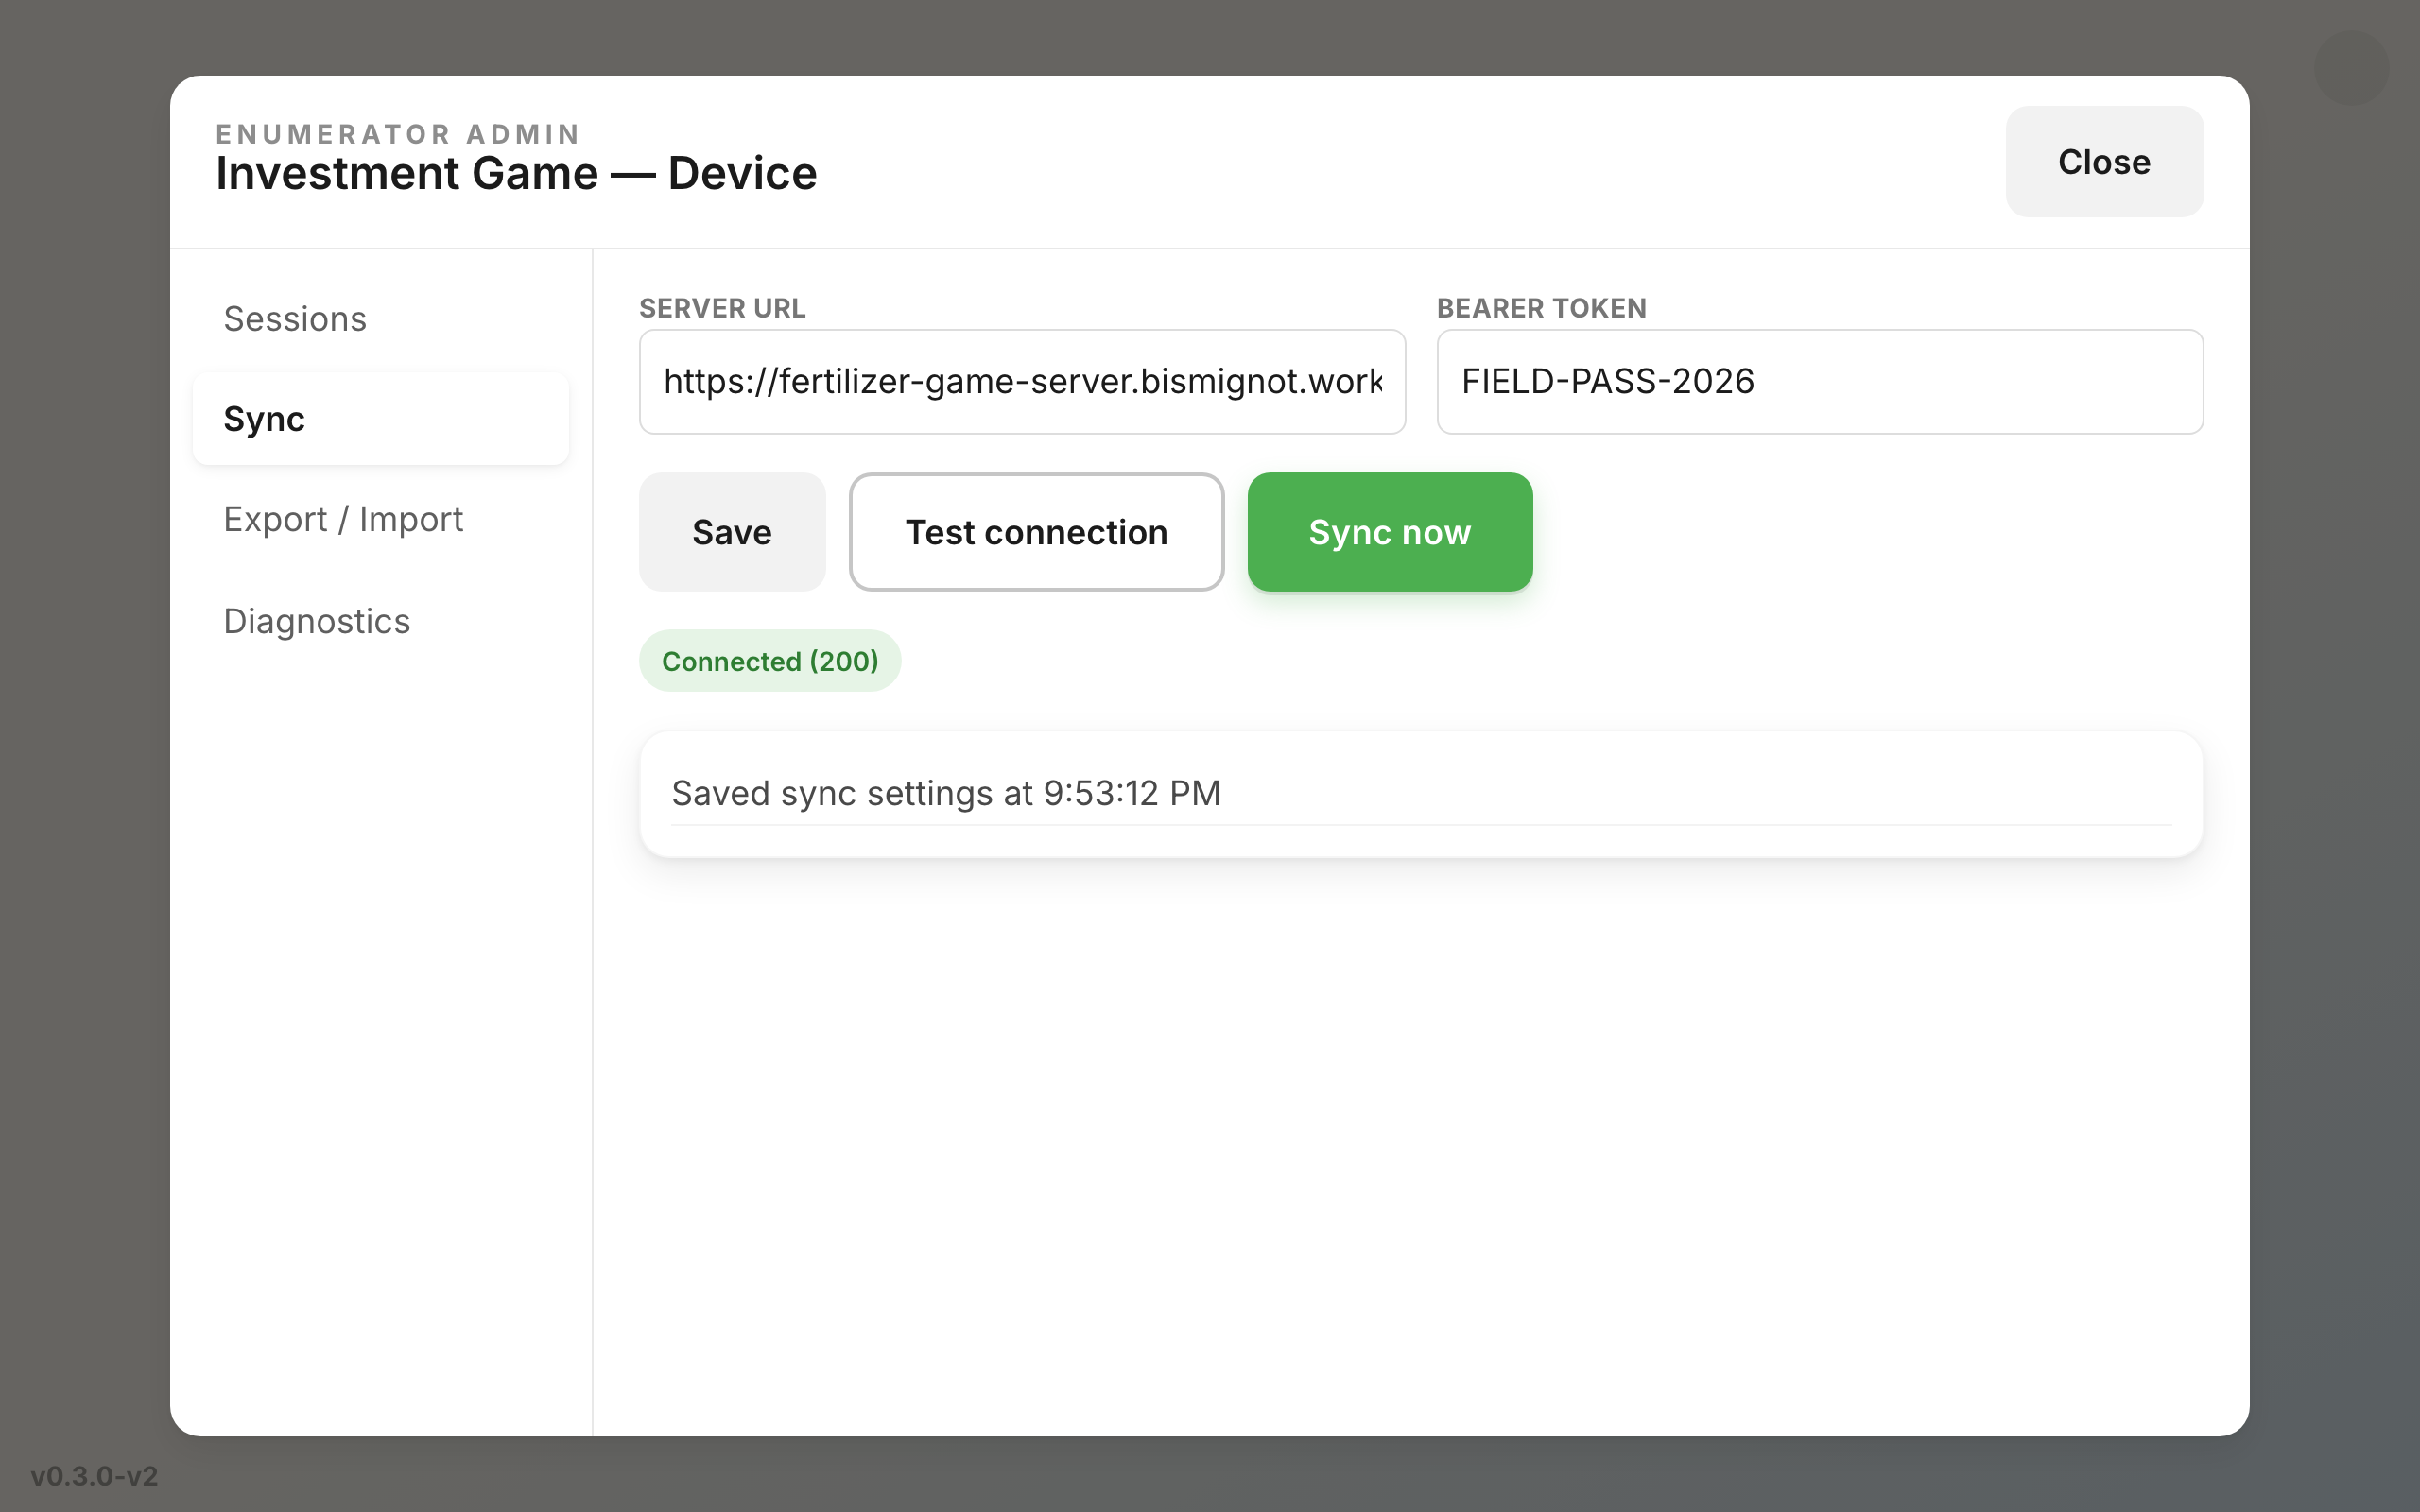
\includegraphics[width=0.7\linewidth]{img/admin-sync.png}}\\[2cm]
{\large\color{inkgrey} CIMMYT Field Experiment Tool}\\[2pt]
{\small\color{inkgrey} Read this together with the farmer-facing ``Fertilizer Game'' guide.}
\vfill
\end{titlepage}

% ===================== 0. WHAT YOU NEED =====================
\section{What you need before the field}

\keybox{Your kit}{%
\begin{itemize}[leftmargin=1.3em,nosep]
  \item A charged \textbf{Android tablet} (landscape).
  \item \textbf{Internet once}, to install the app and to sync data (mobile data or wifi).
  \item The \textbf{Server (sync) address} --- e.g. \texttt{https://fertilizer-game-server.bismignot.workers.dev}
  \item The \textbf{sync token / password} your study coordinator gave you (keep it private).
  \item The \textbf{Admin PIN} (default \texttt{1234}, unless your coordinator changed it).
  \item Your \textbf{Enumerator ID} and the \textbf{list of Participant IDs} for the day.
\end{itemize}}

% ===================== 1. SET UP THE TABLET =====================
\section{Set up the tablet (do this once)}

\subsection{Step 1 --- Install the app}
\begin{enumerate}[leftmargin=1.5em]
  \item Connect the tablet to the internet.
  \item Open \textbf{Chrome} and go to the game's web address (the \emph{app} address, not the server address).
  \item In the Chrome menu (\,$\vdots$\,) choose \textbf{``Add to Home screen''} / \textbf{``Install app''}.
  \item Open the app once and let it finish loading. It now stores everything on the tablet and
  \textbf{works fully offline} --- you do not need internet to run sessions.
\end{enumerate}

\screenshot{img/01-welcome.png}{The Welcome screen. This is the ``home'' of the app. You always start
and return here.}

\subsection{Step 2 --- Open the Admin panel}
The Admin panel is for you, the enumerator --- not the farmer. Open it from the Welcome screen by either:
\begin{itemize}[leftmargin=1.4em,nosep]
  \item pressing the screen with \textbf{four fingers} and holding briefly, or
  \item tapping the small circle in the \textbf{top-right corner}.
\end{itemize}
Then enter the \textbf{PIN} and tap \textbf{Unlock}.

\smallshot{img/admin-pin.png}{Enter the Admin PIN (default \texttt{1234}).}

\subsection{Step 3 --- Configure syncing}
Go to the \textbf{Sync} tab and:
\begin{enumerate}[leftmargin=1.5em]
  \item Type the \textbf{Server URL} and the \textbf{Bearer token} (your sync password).
  \item Tap \textbf{Save}.
  \item Tap \textbf{Test connection}. You should see \textbf{\color{leafgreen}Connected (200)}.
\end{enumerate}

\screenshot{img/admin-sync.png}{The Sync tab, set up correctly. Save first, then Test connection ---
\textbf{\color{leafgreen}Connected (200)} means the tablet can reach the server.}

\subsection{Step 4 --- Quick checks (optional but recommended)}
\begin{center}
\begin{minipage}{0.49\linewidth}\centering
\setlength{\fboxsep}{0pt}\setlength{\fboxrule}{0.6pt}%
\fcolorbox{black!25}{white}{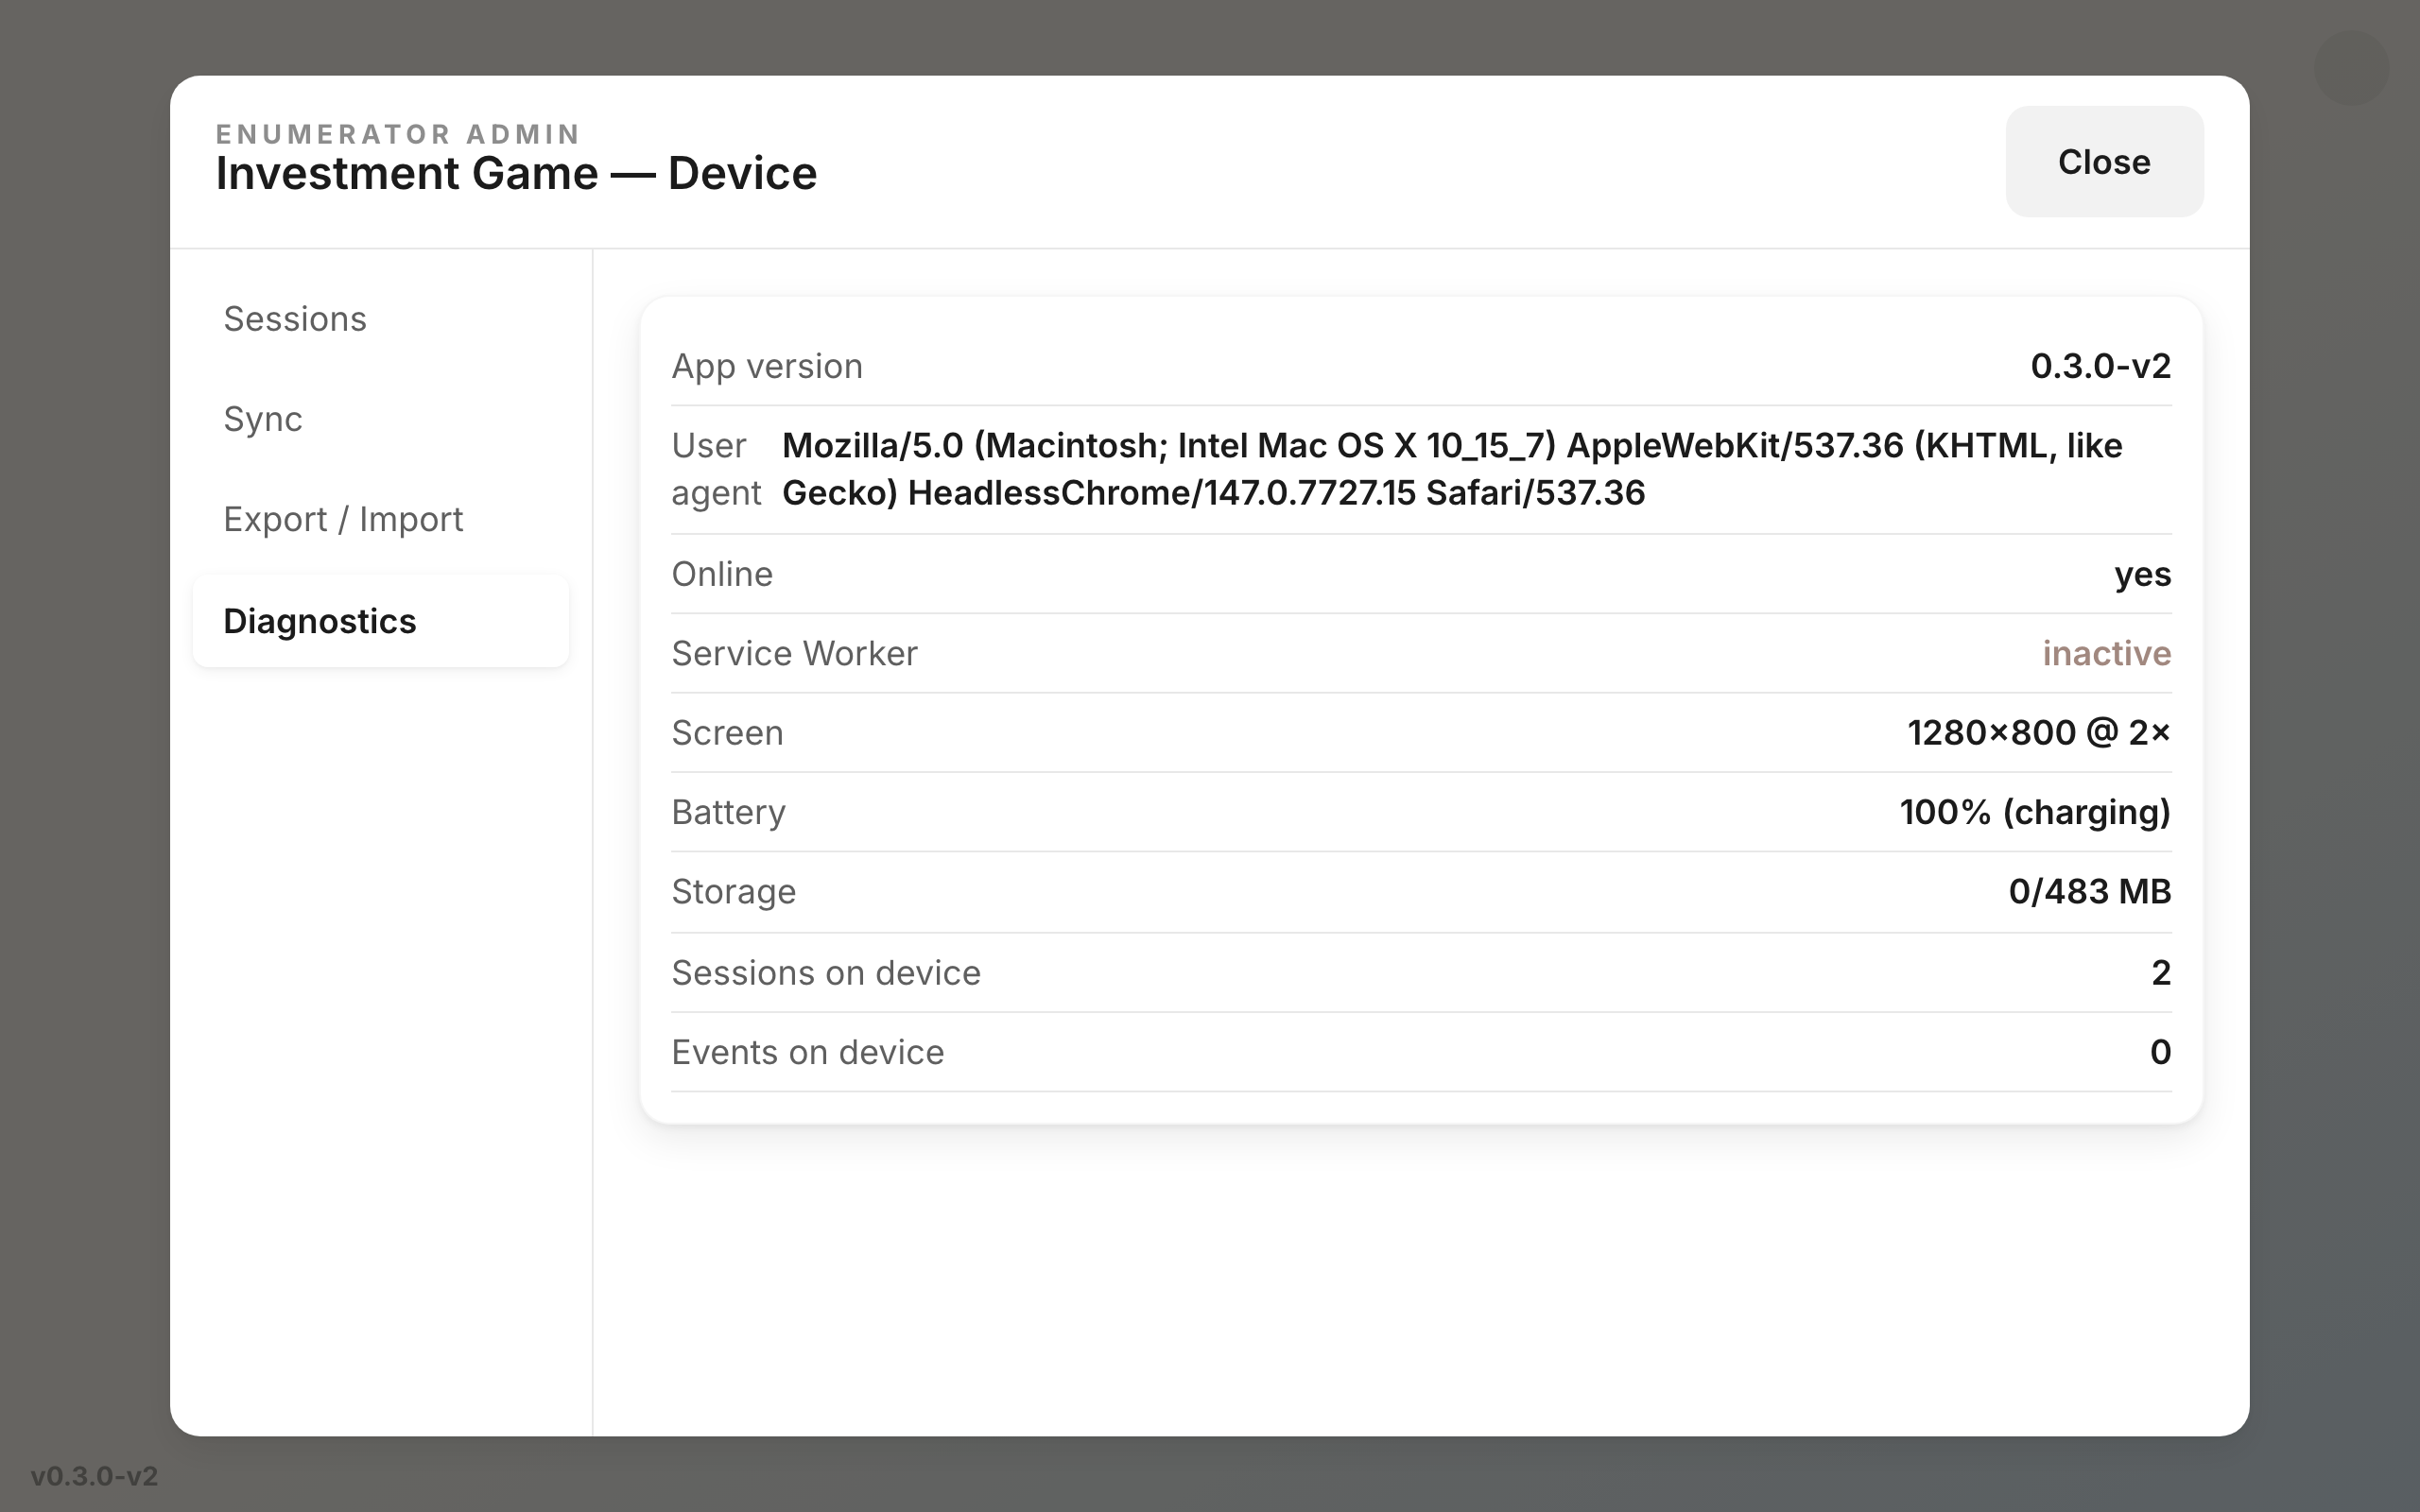
\includegraphics[width=\linewidth]{img/admin-diagnostics.png}}\\[2pt]
{\small\itshape\color{inkgrey} \textbf{Diagnostics} --- check the app is offline-ready,
storage is healthy, and battery is fine.}
\end{minipage}\hfill
\begin{minipage}{0.49\linewidth}\centering
\setlength{\fboxsep}{0pt}\setlength{\fboxrule}{0.6pt}%
\fcolorbox{black!25}{white}{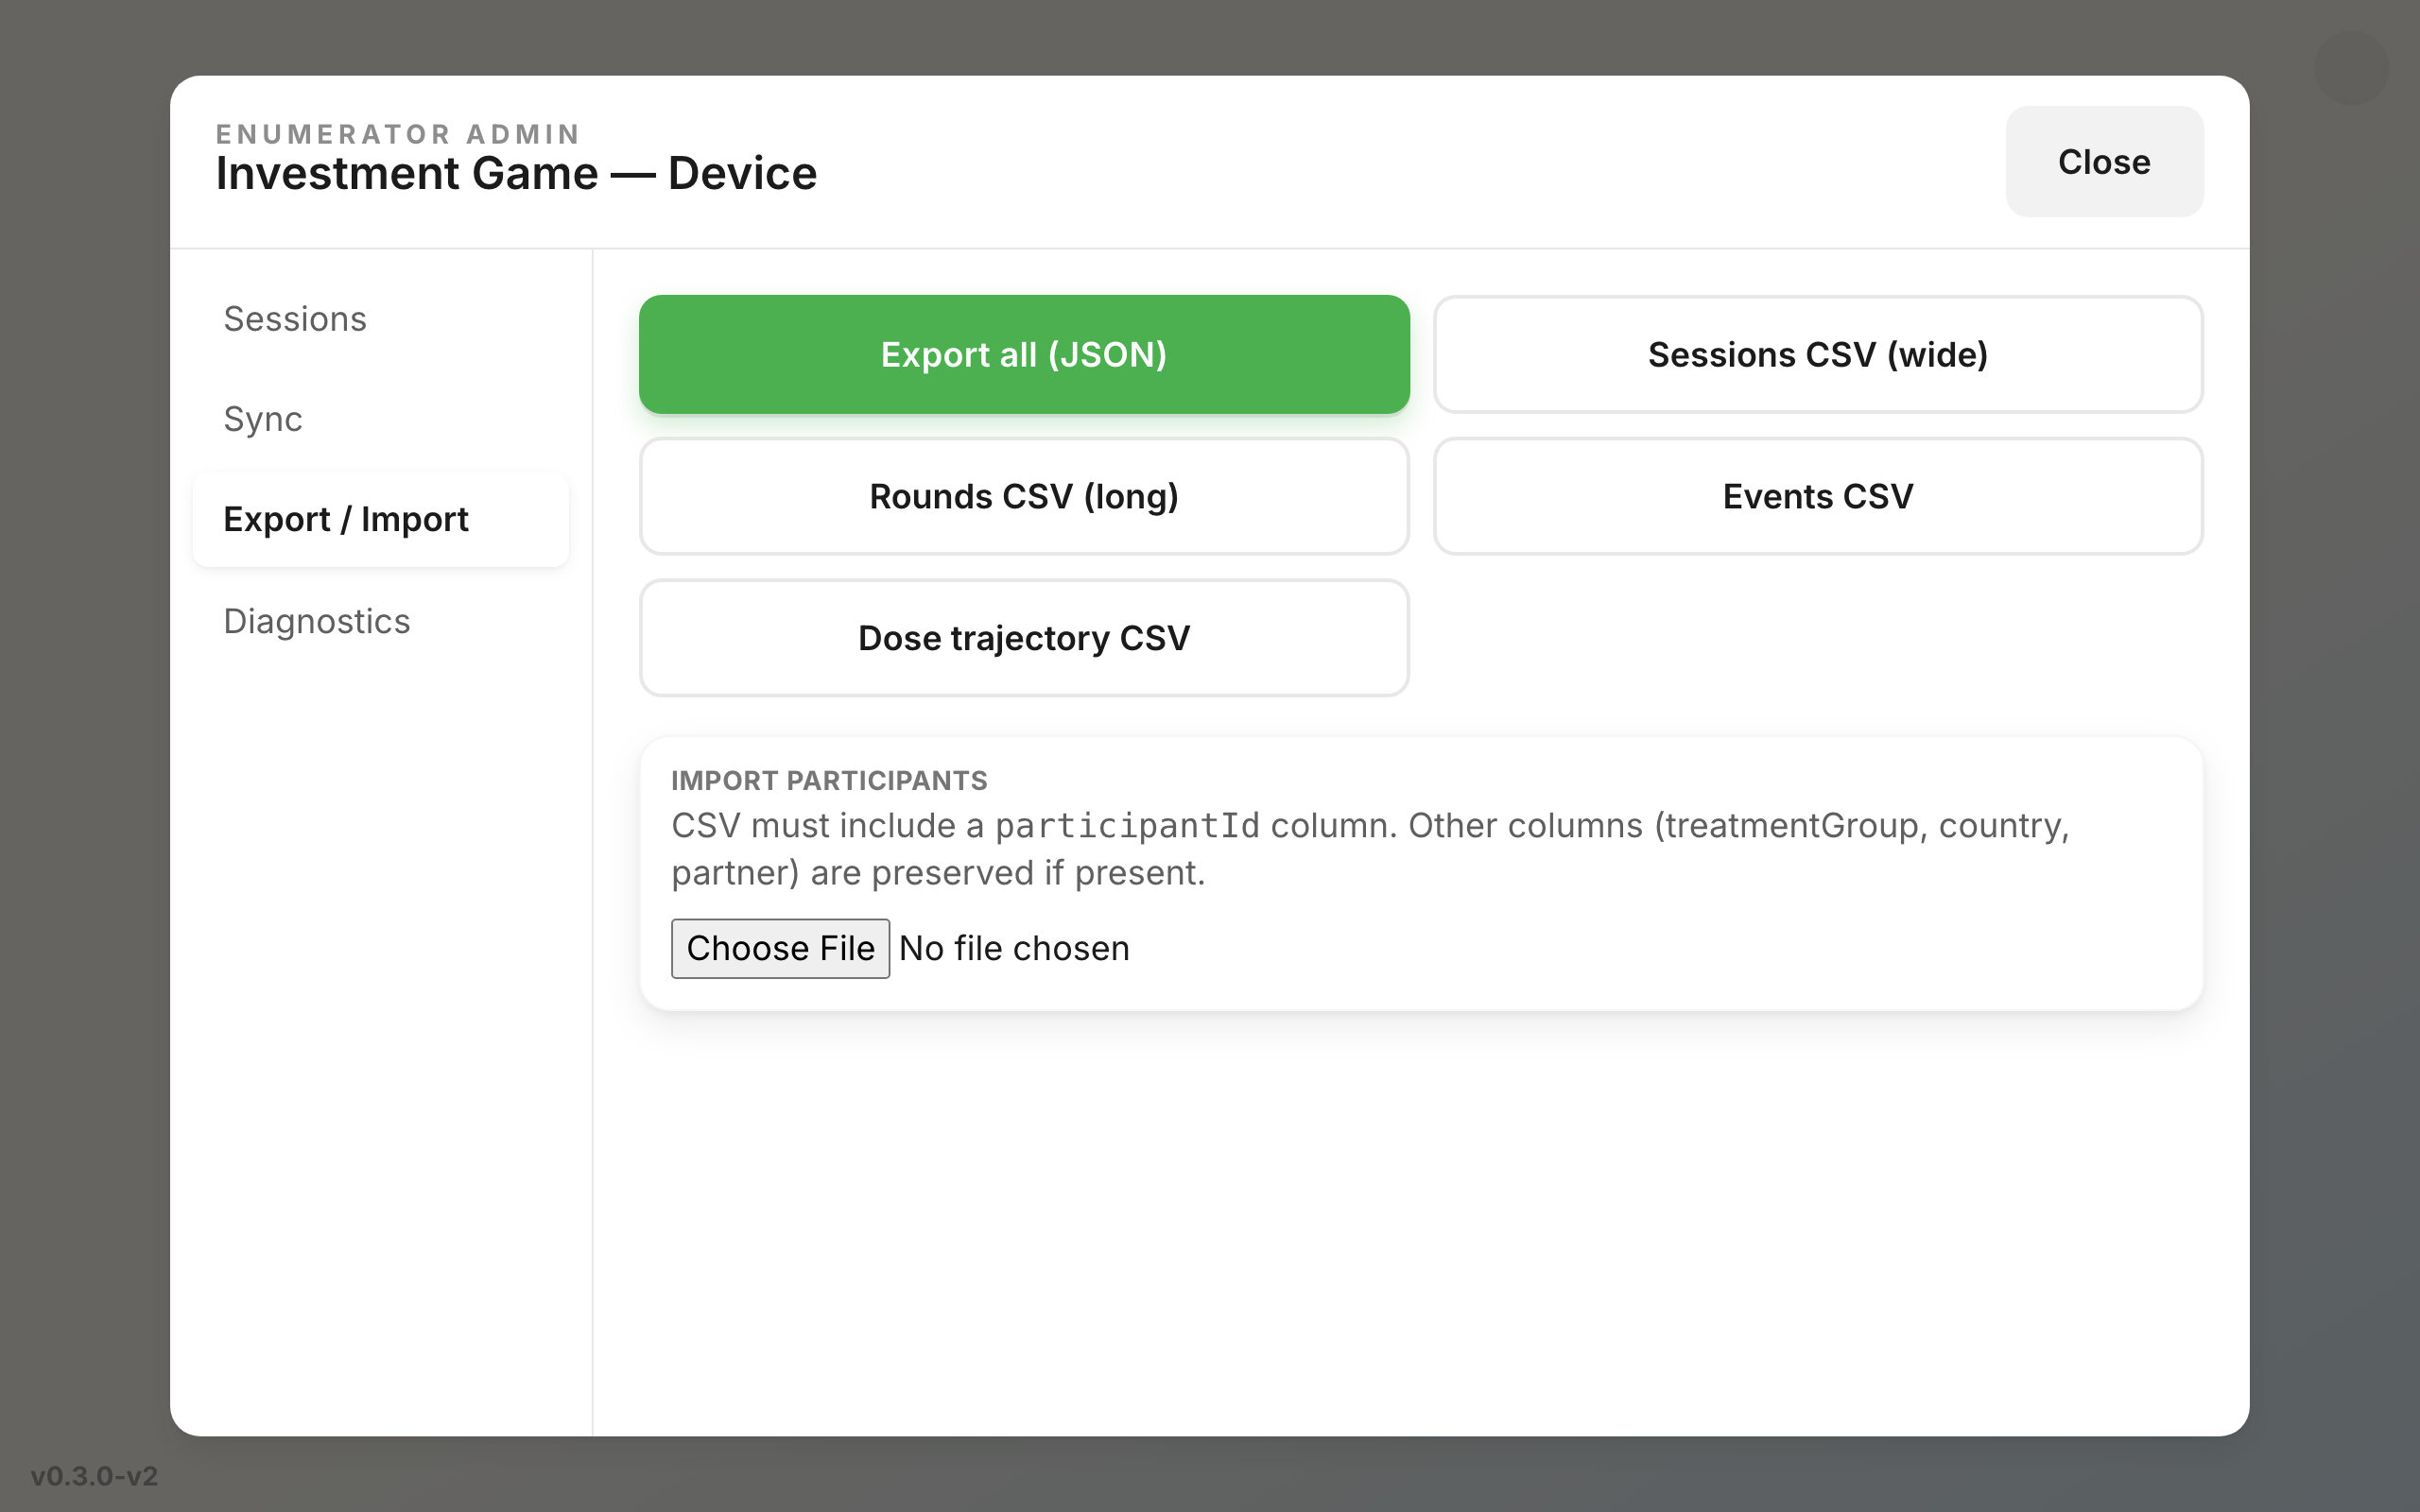
\includegraphics[width=\linewidth]{img/admin-export.png}}\\[2pt]
{\small\itshape\color{inkgrey} \textbf{Export / Import} --- import the participant list (CSV),
and later export data as a backup.}
\end{minipage}
\end{center}

Tap \textbf{Close} to leave the Admin panel.

% ===================== 2. RUN A SESSION =====================
\section{Run a session with a participant}

\subsection{Step 1 --- Start the session}
On the Welcome screen tap \textbf{Begin}. Fill in:
\begin{itemize}[leftmargin=1.4em,nosep]
  \item \textbf{Participant ID} (from your list --- this is what links the game to the baseline survey),
  \item \textbf{Enumerator ID} (yours).
\end{itemize}
The token-to-Naira rate is pre-filled. Then tap \textbf{Start session}.

\screenshot{img/admin-setup.png}{The setup form. The Participant ID is important: it decides the
(random but reproducible) rain and price results, so the session can be checked later.}

\subsection{Step 2 --- The participant plays}
The participant now: chooses the \textbf{language}, sees a short \textbf{picture lesson} about chance,
plays \textbf{1 practice season}, then \textbf{10 real seasons}. Each season they read the rain \& price
outlook and choose how much fertilizer to buy. (See the separate \emph{farmer} guide for how the game works.)

\warnbox{Your job during play}{%
Read or explain the screens if asked, and make sure the participant understands the pictures --- but
\textbf{never tell them how much fertilizer to choose}. The whole point is to record \emph{their} decision.
Let them tap the buttons themselves where possible.}

\subsection{Step 3 --- Pay the participant}
At the end you see \textbf{Your final earnings}: the tokens from each of the 10 seasons, the total,
and the amount in \textbf{Naira (NGN)}. \textbf{Pay the participant that Naira amount.}

\screenshot{img/final-payout.png}{The final earnings screen. Here the total is \textbf{236 tokens =
2{,}356 NGN}. Pay the Naira figure shown. Tap \textbf{Continue} and the ``thank you'' screen ends
the session.}

% ===================== 3. NEXT PARTICIPANT =====================
\section{Start the next participant {\normalsize(read carefully)}}

When you reach the ``thank you'' screen, the participant is finished and \textbf{their data is already
saved on the tablet}.

\keybox{To start the next participant}{%
Tap the \textbf{Next participant} button on the ``thank you'' screen. It takes you straight to the setup
form for the next person and \textbf{keeps all the data from earlier participants} on the tablet.
(If the app was closed, just reopen it --- it returns to Welcome with the data kept.) You can run many
participants on one tablet this way before syncing.}

\dangerbox{Do NOT tap the grey ``Reset'' button to move on}{%
The grey \textbf{\color{dangerred}$\circlearrowright$ Reset} button (bottom of the screen)
\textbf{erases EVERY session stored on the tablet}. It is only for wiping a tablet \emph{after} the data
has been safely synced, or for discarding a test. \textbf{If you tap it before syncing, that data is gone.}
Ask your coordinator to switch this button off for fieldwork.}

\subsection{If the tablet switches off or the app closes during a session}
Do not worry --- just \textbf{reopen the app}. It \textbf{resumes the unfinished session exactly where
it stopped}. Nothing is lost. (A finished session does not resume; the app simply goes to Welcome.)

% ===================== 4. SYNC =====================
\section{Send the data to the server (syncing)}

Sessions stay on the tablet until you sync them. Sync \textbf{whenever you have internet} --- at minimum
at the \textbf{end of each day}.

\begin{enumerate}[leftmargin=1.5em]
  \item Get the tablet online (wifi or mobile data).
  \item From \textbf{Welcome} open the \textbf{Admin} panel $\rightarrow$ \textbf{Sync} tab.
  \item Tap \textbf{Sync now}. Each completed session uploads (\emph{syncing} $\rightarrow$ \emph{synced}).
\end{enumerate}

\keybox{Good to know}{%
\begin{itemize}[leftmargin=1.3em,nosep]
  \item \textbf{Safe to repeat.} Tapping Sync now again never creates duplicates --- already-sent
  sessions are simply skipped.
  \item \textbf{Only finished sessions} are sent. An unfinished session waits until it is completed.
  \item \textbf{Nothing is deleted} from the tablet by syncing --- the sessions stay as a backup,
  now marked \emph{synced}.
  \item \textbf{If it fails} (weak signal), it marks the session \emph{failed} and will retry the next
  time you tap Sync now.
\end{itemize}}

\subsection{Check that it worked}
Open the \textbf{Sessions} tab. The \textbf{Sync} column should show \textbf{\color{leafgreen}synced}
for finished sessions.

\screenshot{img/admin-sessions.png}{The Sessions list. Each session shows the participant, group, tokens,
and a sync status: \textbf{\color{leafgreen}synced} (on the server) or \textbf{pending} (still only on the
tablet). Sync again until everything shows \emph{synced}.}

\subsection{No internet for a long time?}
The data is safe on the tablet --- sync when you next get a signal. If you must hand the data over without
internet, use \textbf{Admin $\rightarrow$ Export / Import} to download the files and give them to your
coordinator.

% ===================== 5. RULES =====================
\section{Golden rules}

\begin{enumerate}[leftmargin=1.5em]
  \item \textbf{To move to the next participant: close and reopen the app.} Never use Reset for this.
  \item \textbf{Sync (or export) before wiping a tablet.} Once data is gone from the tablet \emph{and}
  not on the server, it cannot be recovered.
  \item \textbf{Sync at the end of every day}, and check the Sessions tab shows \emph{synced}.
  \item \textbf{Never tell a participant what to choose.} Record their own decisions.
  \item \textbf{Keep the PIN and the sync token private.}
  \item \textbf{Keep the tablet charged} --- check the battery in Diagnostics.
\end{enumerate}

% ===================== 6. TROUBLESHOOTING =====================
\section{Troubleshooting}

\begin{center}
\begin{tabular}{@{}p{0.42\linewidth}p{0.52\linewidth}@{}}
\toprule
\textbf{Problem} & \textbf{What to do} \\
\midrule
Test connection / Sync fails with \emph{401} or \emph{403} & Wrong or empty token. Re-type the
Bearer token in the Sync tab, Save, and test again. \\
Test connection fails with no number & The tablet has no internet, or the server address is wrong.
Check your signal and the Server URL. \\
``Sync'' says some sessions \emph{failed} & Weak signal during upload. Get a better connection and
tap \textbf{Sync now} again --- it retries automatically. \\
The app won't open / blank screen & Reopen it. If it was never loaded online first, connect to
internet once and reload. \\
A session seems stuck or the tablet restarted & Reopen the app; it resumes the unfinished session. \\
I tapped Reset by mistake & Sessions already \emph{synced} are safe on the server. Anything only on the
tablet and not yet synced is lost --- tell your coordinator. \\
\bottomrule
\end{tabular}
\end{center}

\vfill
\begin{center}
{\small\color{inkgrey} CIMMYT Fertilizer Risk-Communication Experiment. Screens shown are the English
version; the game is also played in Hausa. Keep this guide with the tablet.}
\end{center}

\end{document}
